\chapter{ساخت تصویر برداری}
\begin{summary}
در این فصل طریقه‌ی ساخت تصویر برداری در نرم‌افزار متلب را توضیح خواهیم داد و یک نمونه از استفاده از آنها را خواهیم دید.
\end{summary}
\section{نمایش یک منحنی}
ابتدا منحنی -یا هر طرح گرافیکی ریاضی‌وار در متلب را- تولید می‌کنیم تا بتوانیم از آن استفاده کنیم. برای این منظور قطعه کد متلب زیر را در نظر می‌گیریم
\begin{latin}
\lstinputlisting[mathescape]{codes/sincos.m}
\end{latin}
طبیعی است که دستورات زیر یک نمودار برایمان تولید می‌کند:
\begin{latin}
\begin{lstlisting}
>> x = 0:.01:4.5;
>> y = sincos(x);
>> plot(x,y);
\end{lstlisting}
\end{latin}

\section{ساخت تصویر برداری}
حال با این فرض که دستورات بخش قبل اجرا شده‌اند و یک فایل تصویری الان روبروی شما باز است، دستور زیر را در متلب وارد می‌کنیم
\begin{latin}
\begin{lstlisting}
print -depsc2 "sincos_long.eps"
\end{lstlisting}
\end{latin}
که در آن \lr{sincos\_long.eps} نام فایلی است که می‌خواهیم تصویر با آن نام ذخیره شود. اکانون اگر به پوشه‌ی جاری متلب بروید، خواهید دید که یک فایل با نام مذکور ساخته شده است. فایل را به پوشه‌ای که فایل‌های لاتک در آن قرار دارند -و شما در آن مشغول نوشتن پایان‌نامه‌تان هستید- انتقال دهید. اکنون با استفاده از دستور زیر، آنرا نمایش دهید:
\begin{latin}
\lstinputlisting[language=TeX]{codes/sample_figure.tex}
\end{latin}
که نتیجه‌ی آن تصویر زیر می‌شود:
\begin{figure}[!h]
\centerline{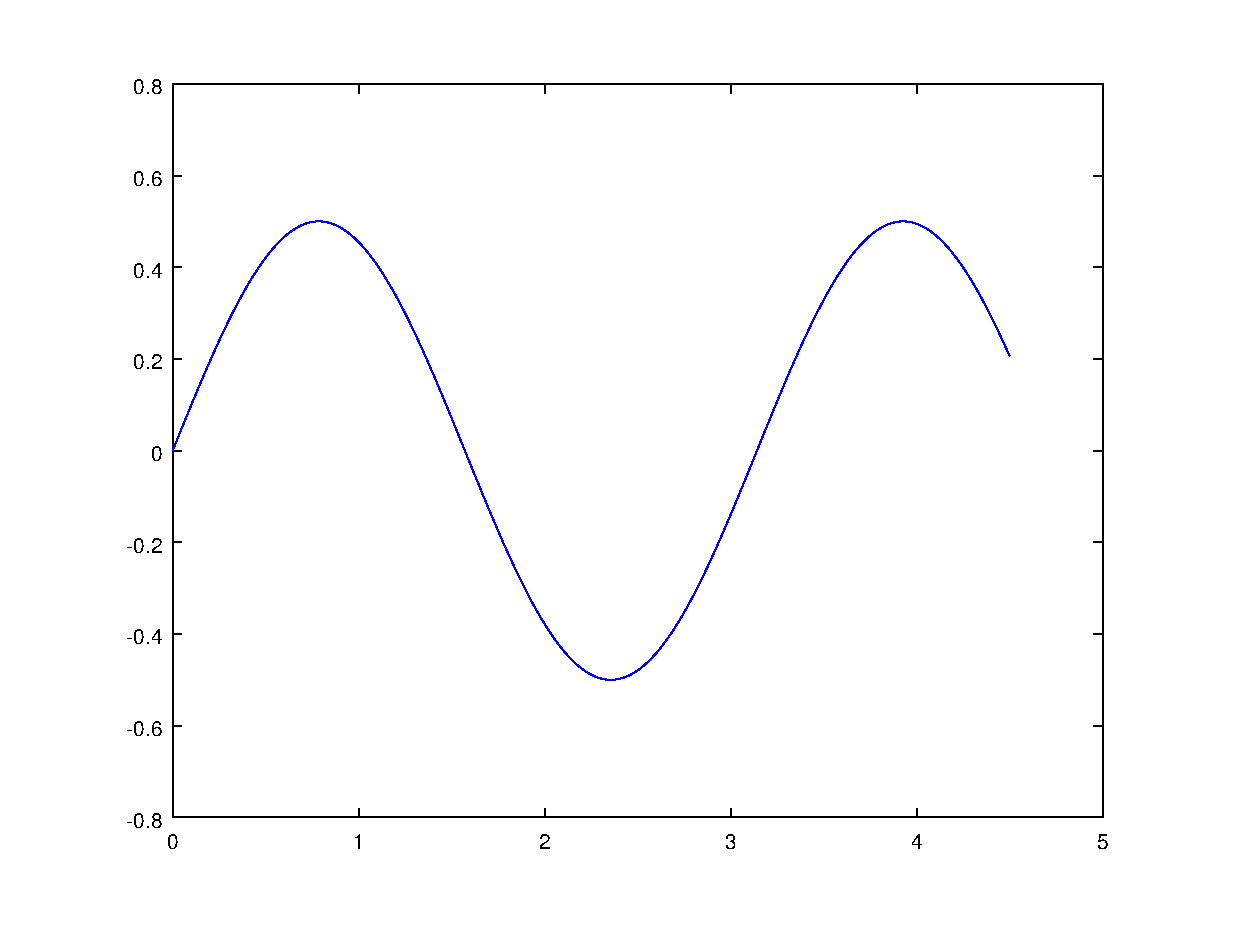
\includegraphics[scale=.45]{sincos_long}}
\caption{تصویر تابع $\sin(x)\times\cos(x)$ که $x\in[0,4.5]$.}
\label{fig:2:sincos_long}
\end{figure}